\subsection{Worker f�r Daten�bermittlung}\label{subsec:Worker}
Der vorliegende Abschnitt befasst sich mit dem Teil der Wissenserwerbskomponente, der als Bindeglied zwischen den Wissenserfassungsmethoden und der Wissensbasis auftritt und in Abbildung \ref{fig:wissenserwerbskomponente} als Schnittstelle f�r die Daten�bermittlung bezeichnet wird. Im Rahmen dieser Arbeit wird der Begriff \glqq{}\textit{Worker}\grqq{} verwendet, der f�r die Auspr�gung dieser Schnittstelle steht. Im Folgenden wird das Konzept hinter dem Worker abstrakt skizziert und im weiteren Verlauf mit der konkreten Implementierung verdeutlicht. Der Anwendungsbereich vom Worker l�sst sich in Abbildung \ref{fig:worker} wie folgt darstellen:
\begin{figure}[H] 
	\centering
	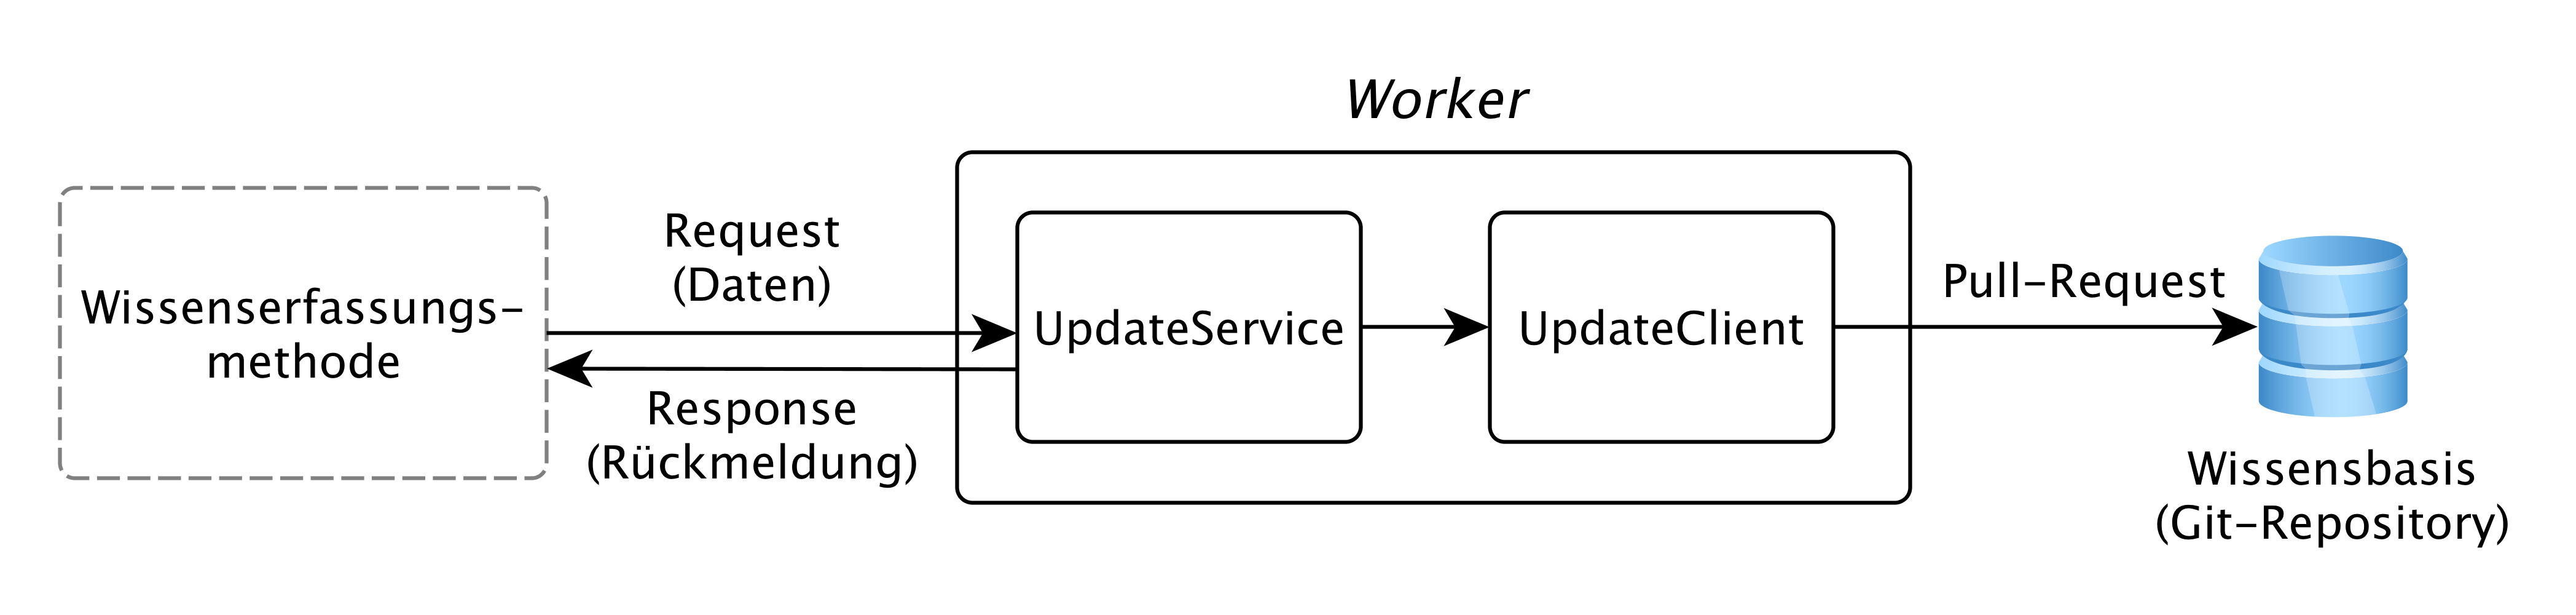
\includegraphics[width=1.0\textwidth]{images/anwendungsbereich_worker.png}
	\caption{Anwendungsbereich vom Worker}
	\label{fig:worker}
\end{figure}
Grunds�tzlich besteht der Worker aus zwei Komponenten, n�mlich \glqq{}\textit{UpdateService}\grqq{} und \glqq{}\textit{UpdateClient}\grqq{}. Die Aufgabe vom UpdateService besteht in der Bereitstellung einer Schnittstelle, die die Daten von au�en aufnimmt und die Daten�bermittlung an den UpdateClient delegiert. Auf der anderen Seite stellt der UpdateClient die Methoden zur Verf�gung, die f�r die Daten�bermittlung zust�ndig sind.\\
Generell l�sst sich der Ablauf gem�� der Abbildung \ref{fig:worker} folgenderma�en beschreiben. Als erstes werden die Daten von der Wissenserfassungsmethode an den UpdateService gesendet. Darauffolgend werden die Daten vom UpdateService verarbeitet und f�r den UpdateClient vorbereitet. Im n�chsten Schritt wird die Aufgabe der Daten�bermittlung an den UpdateClient delegiert. Der UpdateClient erstellt die Anfrage an die Wissensbasis und teilt die Antwort dem UpdateService mit. Anschlie�end verschickt der UpdateService die R�ckmeldung an die Wissenserfassungsmethode.\\ 
Im Weiteren wird die Wissenstr�gerschnittstelle aus dem Abschnitt \ref{subsec:Wissenstr�gerschnittstelle} als Wissenserfassungsmethode betrachtet. Die Wissensbasis stellt das Git-Repository von \textit{PaaSfinder} dar, das von einem Bot-Account auf Github \glqq{}geforkt\grqq{} wird\footnote{https://github.com/update-bot/paas-profiles}. In anderen Worten wird das urspr�ngliche Git-Repository von \textit{PaaSfinder} kopiert, sodass der Bot-Account einen schreibenden Zugriff auf die Wissensbasis hat.\\
Technisch gesehen erfolgt der Nachrichtenaustausch zwischen Wissenserfassungsmethode, dem Worker und der Wissensbasis auf Basis von \ac{HTTP}\footnote{https://www.w3.org/Protocols} und \ac{REST} Architekturstil, der urspr�nglich aus der Dissertation von Fielding \cite{fielding2000} stammt. Das zentrale Konzept von REST basiert auf Ressourcen, die im globalen Raum mithilfe von \ac{URI}\footnote{https://tools.ietf.org/html/rfc3986} eindeutig identifiziert werden \cite[S.11,35]{tilkov2015}. Zusammenfassend wird ein PaaS-Profil als Ressource an REST API per HTTP Protokoll verschickt.\\
Wie bereits angedeutet wurde, implementiert der UpdateService die REST Schnittstelle, die die Daten von au�en entgegennimmt. In diesem Fall wurde das Spark\footnote{http://sparkjava.com} Framework als Technologie zur Umsetzung der Schnittstelle verwendet. Die Schnittstelle stellt die Route \glqq{}/vendor\grqq{} dar, die vom Typ POST\footnote{https://tools.ietf.org/html/rfc7231\#section-4.3.3} ist und die Daten in JSON Format akzeptiert. F�r das Parsen und Erstellen der JSON-Objekte wurde die Gson\footnote{https://sites.google.com/site/gson/Home} Bibliothek verwendet. In Bezug auf die Notation wird die Route in Listing \ref{service} abgebildet.
\begin{lstlisting}[basicstyle=\ttfamily, label=service,
					captionpos=b, caption={\glqq{}/vendor\grqq{} Route}]
post("/vendor", "application/json", (request, response) -> {
   ...
});
\end{lstlisting}
Der Ablauf der Pull-Request-Erstellung besteht aus folgenden Schritten:
\begin{enumerate}
\item Branch erstellen
\item Das Profil im erstellten Branch aktualisieren
\item Pull-Request erstellen
\end{enumerate}
Die oben beschriebenen Schritte werden als Anfragen an die Github API\footnote{https://developer.github.com/v3} umgesetzt. F�r das Bilden der Anfragen wird intern der HTTP Client von OkHttp\footnote{https://square.github.io/okhttp} verwendet. Die Schnittstelle vom UpdateClient erwartet als Eingabeparameter die Nachricht, die an das Repository gesendet werden soll. Bei einer Nachricht handelt es sich entweder um einen Branch, eine File oder einen PullRequest. Zusammenfassend werden die Anfragen in Listing \ref{client} skizziert:
\begin{lstlisting}[basicstyle=\ttfamily, label=client,
					captionpos=b, caption={Schnittstelle vom UpdateClient}]
class UpdateClient {
    void postBranch(Branch branch) {...}

    void putFile(File file) {...}

    void postPullRequest(PullRequest pullRequest) {...}
}
\end{lstlisting}
Im Abschnitt \ref{subsec:Wissenstr�gerschnittstelle} wurde das Profil \glqq{}Heroku\grqq{} aktualisiert. Sobald der Benutzer auf \glqq{}Submit\grqq{} klickt, werden die Daten als JSON in der POST-Anfrage an den Worker gesendet, n�mlich an die Schnittstelle vom UpdateService. Im besten Fall werden die Nachrichten (Branch, File und PullRequest) erfolgreich erstellt und vom UpdateClient an das Git-Repository �bermittelt (siehe Abbildung \ref{fig:pull-requests}).
\begin{figure}[H] 
	\centering
	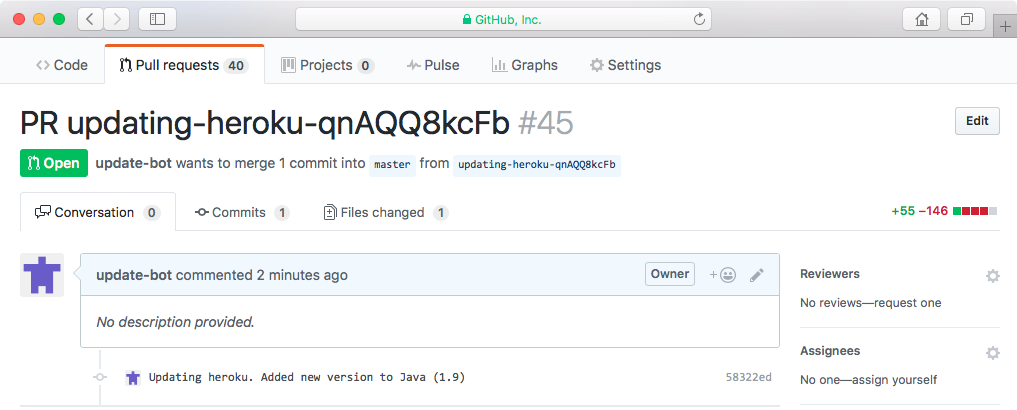
\includegraphics[width=0.9\textwidth]{images/pull-requests.png}
	\caption{Github Pull-Requests Ansicht}
	\label{fig:pull-requests}
\end{figure}
In der Detailansicht werden ebenso die �nderungen explizit gezeigt. Dabei werden die gel�schten Zeilen als rot markiert und die dazugekommenen als gr�n. Im Beisiel von \glqq{}Heroku\grqq{} wird das in Abbildung \ref{fig:pull-request-detail} verdeutlicht.
\begin{figure}[H] 
	\centering
	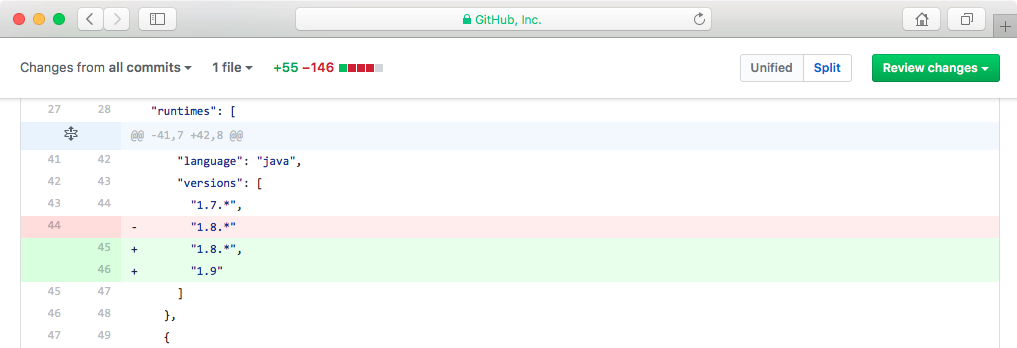
\includegraphics[width=0.9\textwidth]{images/pull-request-detail.png}
	\caption{Heroku Pull Request}
	\label{fig:pull-request-detail}
\end{figure}
Ausgehend vom erfolgreichen �bermitteln der Daten an das Repository schickt der UpdateService die Antwort (Response) mit dem Statuscode 200 (\glqq{}OK\grqq{}) an die Wissenserfassungsmethode zur�ck. In Bezug auf die Fehlerbehandlung wird ein logischer Schritt (Branch erstellen, File aktualisieren und PullRequest erstellen) in einem eigenen try-catch-Block ausgef�hrt, sodass der Client eine aussagekr�ftige Fehlermeldung bekommt.